\documentclass[12pt]{article}
\usepackage[margin=1in]{geometry}
\usepackage{graphicx}
\usepackage{amsmath}

\bibliographystyle{plain}

\begin{document}

\title{Independent Study CS499}
\author{Art Grichine}
\date{\today}

\maketitle	

%==================== Introduction ====================

\section*{Introduction}
Every semester, The Computer Science department at California State University, Fullerton faces 
oversubscribed courses. This problem affects both the students and the staff in the department. 

For the students of Cal State Fullerton, oversubscribed courses lead to uncertainty during registration, 
inability to fill required course load, and even delay in graduation. Sometimes additional courses are 
added or a student is chosen from a wait list. However, for every student that is selected from the 
waitlist, countless others are unable to take the necessary class. I have personally experienced this 
problem and have been at the mercy of the department to make room for me.

Currently, course demand is based on the department's intuition. This leads to difficult decisions 
regarding what courses the department should offer and how many sections to offer per course. 
Furthermore, these decisions must be made by the department several months before the semester 
to ensure staff availability thereby leading to difficulties with last minute additions due to demand.

By applying machine learning principles (e .g. regression, neural networks), Dr. Wortman and I believe 
that it should be possible to predict the demand for each course offered by the department.

%==================== Review of Literature ====================

\section*{Review of Literature}
While researching the enrollment forecasting topic, it came as a surprise that there was not much literature 
covering this topic. Most research in this domain focuses on enrollment in the higher-education system 
rather than dealing with the individual department. Two articles were found from 1973 and 1975. However, 
a more recent paper from 2005 by Kraft and Jarvis \cite{kraft2005adaptive} addresses these papers. 
Kraft and Jarvis attempt to solve the enrollment forecasting problem through a seat release system which 
attempts to predict the number of seats needed for a given section. They identify student characteristics 
that are significant in predicting course enrollment such as first-time vs. transfer student and pass/fail rates 
of courses. Data from the previous three years is used as a historical estimation and verification for the 
parameters in the seat release model. The model output reports the minimum, mean, and maximum 
predicted values for an individual course. The authors argued that their model proved to be accurate and 
robust.

More recently, a lecture from University of Missouri-Columbia in 2010 by Felts and Ehlert \cite{LectureMU} 
presented an approach which considers a ratio of student demand for a course to the total students in the 
available population. They use the historical calculated student demand correlation value and apply it to the 
new student population. The output is the new predicted student demand. 

%==================== Methods ====================

\section*{Methods}
Course enrollment models not using department intuition consider regression analysis to determine course 
demand. However, regression models may have large error when department policies change regarding 
curriculum hours and courses required. Also, the student progression through the courses can vary 
significantly due to individual professor grading. The model used for this study considers historical course 
grades to predict the amount of students that will pass the course and continue and course demand which
is gathered through a questionnaire.

\subsection*{Data}
Student data was generated through a Python script called \texttt{Dataset\_Generator.py}. The dataset 
generator used the libraries Pandas, Numpy, and MatPlotLib to generate, manipulate, and store data to a .csv file
which is then read and used by other programs. This dataset generator was created due to the inability to timely 
gather needed data for this project. Instead, a Python dictionary of courses was created to hold all 
undergraduate courses offered by the department of Computer Science at Cal State Fullerton. The main 
program \texttt{Course\_Progression.py} calls methods belonging to the \texttt{Dataset\_Generator.py} 
program to generate data for its computation. The functions \texttt{handle\_grades()} and \texttt{handle\_demand()} 
are called from the main menu of \texttt{Course\_Progression.py}. Depending on the user's menu selection,
the \texttt{Dataset\_Generator.py} methods are used to generate the appropriate data. The user also has the
option of loading their own data into the program.

\subsubsection*{Demand Data}
The \texttt{handle\_demand()} function in \texttt{Course\_Progression.py} asks the user whether they would like
to load demand data or if they would like to generate a dataset. Loading data is a trivial action in which the 
Pandas \texttt{read\_csv()} method is used and a Pandas data frame containing the file contents is returned to 
the main menu. The generate demand option calls the \texttt{generate\_demand()} method from the
\texttt{Dataset\_Generator.py} program. This method uses the default value of \texttt{students=1000} and 
creates a Pandas data frame of current courses and wanted courses for 1000 individual student. This is done 
to emulate a questionnaire which would ask students which courses they are currently enrolled in and which 
courses they would like to take next semester. 

As the Pandas data frame for student demand is being created, list Python's list comprehension is used to 
generate individual samples of which courses a student is currently taking and what they would like to take.
In the list comprehension, the \texttt{generate\_samples(students)} function is called to generate individual 
samples. The \texttt{generate\_samples(students)} function iterates through the range of the amount of samples 
needed (in this case \texttt{students=1000}j and appends a random sample of courses from the \texttt{cs\_courses}
dictionary into a list of lists (a list of 1000 students each with their own preference). The Numpy 
\texttt{random.choice()} method is used to vary the amounts of courses a student is taking. This method 
takes a parameter \texttt{p} which can be set to a probability distribution for the values chosen. Here, we would
like to select between one to six courses for each student (simulating a student course load). However, in most
cases it is likely that the student is taking between three to five courses and not one or six courses. Thus, using 
\texttt{np.random.choice()} we can set a higher probability at choosing values of three to five and less at
choosing the values of one and six. Once the choice of how many courses to sample from \texttt{cs\_courses} 
is returned. The \texttt{random.sample()} function is called to choose a random sample of the \texttt{cs\_courses}
dictionary. The samples are then returned to the data frame of current courses and wanted courses in the 
\texttt{generate\_demand()} method and the data frame is saved to a demand$\_$data.csv file and returned to the caller.

\subsubsection*{Grade Data}
Just as with demand data, the grade data must be loaded or generated for this program. When the user 
selects from the main menu the option generate or load student demand data, the \texttt{handle\_grades()} function
is called and the user is prompted to select if they would like to load or generate grade distribution data for their run. 
If the user chooses to load grades from their own dataset, they will be asked how many grade datasets they
would like to load. The user will then enter the names for the .csv file in the working directory one by one until
the grades are successfully loaded. However, if the user would like to generate grade distribution data, the 
user is asked how many datasets would they like to generate and then the users input is passed to the 
\texttt{generate\_grades()} method from \texttt{Dataset\_Generator.py} to generate and load the necessary
data frame.

The \texttt{generate\_grades()} method from \texttt{Dataset\_Generator.py} program takes one parameter 
which contains the amount of records needed. It returns a list of data frames which contain grade distributions 
for each simulated semester. Each individual data frame contains all courses offered by the undergraduate 
program at the Computer Science Department at Cal State Fullerton. A loop which iterates over the range of
records needed calls the \texttt{assign\_grades()} function which returns a grade distribution for all courses. 
This result is then appended to the list of data frames and the file is saved to the working directory for record. 
Once the loop is complete, the list of data frames is returned to the caller.

The \texttt{assign\_grades()} function creates a random Gaussian (normal) distribution by calling Numpy's 
\texttt{np.random.normal()} method. This method takes two parameters, mean or $\mu$ and standard deviation or 
$\sigma$. The mean grade value of $\mu=75$ and the standard 
deviation value of $\sigma=10$ was used to generate the course grades. However, with course grade distribution 
information this value can be trained to more adequately resemble each individual course distribution. In Figure 
\ref{fig:fig1}, we see a histogram of the grade distribution generated for an individual course plotted with a probability
density function (PDF) line to demonstrate ideal distribution. These grade values are recorded for a given course 
and then saved. This process is repeated until all courses have grades. Note that each course has its own unique 
grade distribution as would be seen in practice. A data frame created from the distribution and then returned to the \
texttt{generate\_grades()} method. The data frame is saved for record and the loop continues. Once the needed 
amount of records is created the list of data frames is returned to the caller.

\begin{figure}[h]
    \centering
    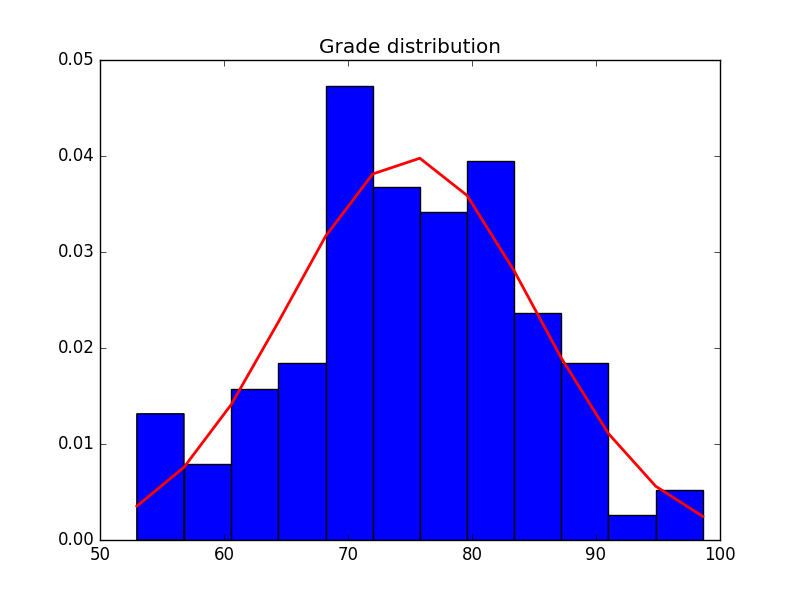
\includegraphics[scale=0.50]{GradeDistribution}
    \caption{Grade Distribution For A Course}
    \label{fig:fig1}
\end{figure}

\subsection*{Forecast}
To forecast data, the user must select the Forecast Enrollment option in the main menu. At least two files must be 
loaded before this option is possible. The demand data as well as the grade distribution data must be in loaded using
the menu before the forecast enrollment option will work. If this option is selected before the necessary data is loaded, 
the user is asked to go back and load or generate the necessary data. When the necessary data is loaded, the 
\texttt{forecast\_enrollment()} function is called and the forecast is computed. When the computation is complete, the 
result is saved to the working directory as forecast.csv and the head and tail of the data frame is shown to the user 
on the command line. The user is then directed back to the main menu where they may run another simulation or 
exit the program.

\subsubsection*{Forecast Enrollment}
When the \texttt{forecast\_enrollement()} function is called by the main menu, it takes the list of data frames containing 
the grade distributions for each course and a data frame which contains the current student courses and demand. The
function then calls the \texttt{grade\_progression()} function which takes the list of grade distributions to process the data.

In the \texttt{grade\_progression()} function, we must extract the amount of passing grades for each course as well as the
total amount of grades assigned. The list of data frames containing the grade distributions for each simulated semester
is enumerated through to extract the sum or passing grades (C- or better) and the sum of total grades assigned to each 
course. These records are aggregated into one data frame which contains all courses offered as well as the passing, total, 
and success ratio for each course. The success ratio is computed by 
$$
\frac{\sum \text{Passing Grades}}{\sum \text{Total Assigned Grades}} = \text{Success Ratio}.
$$
This data frame is then saved to grade\_stats.csv and returned to the \texttt{forecast\_enrollment()} function. 

Next, the \texttt{forecast\_enrollment()} function must also extract the necessary information from the student records. 
The \texttt{student\_demand()} function is called and the data frame containing the student records is passed as 
a parameter. Student demand must go through the records of every individual student generated and count the 
courses that the students are currently in and the ones that are demanded. The \texttt{student\_demand()} function 
counts and aggregates all of the student demand information into a dataframe which contains the course number, 
course name, amount currently enrolled, and amount requesting course. The data frame is then saved as 
student\_stats.csv and returned to the \texttt{forecast\_enrollment()} function.

The \texttt{forecast\_enrollment()} function then creates final data frame which will contain the forecasted contents as 
well as other important data. The course names and numbers are added to the data frame. The column containing 
the amount of students currently enrolled in each course is also added. Finally, the amount of students currently enrolled
in each course is multiplied by the success ratio in the grade distribution data frame. The column containing the 
course demand is transferred to the data frame and the head and tail of the contents are displayed to the screen. The 
data frame contents are then saved to the working directory as forecast.csv and the user is directed back to the main menu.

%==================== Results ====================

\section*{Results}
The program created works as intended. It is robust and did not crash during testing. The results of this study 
cannot be determined because of the inability to measure which courses are ultimately taken. This simulation 
would not only need to generate data for the students and grades but would have to also generated enrollment 
information for the following semester to compute error. However, there is no objective way to compute these
values. Therefore, we cannot objectively judge the performance of this approach. 
An example of the output can be seen in Figure \ref{fig:fig2} as well as a full run in Figure \ref{fig:fig3} at the end 
of this document.
\begin{figure}[h]
    \centering
    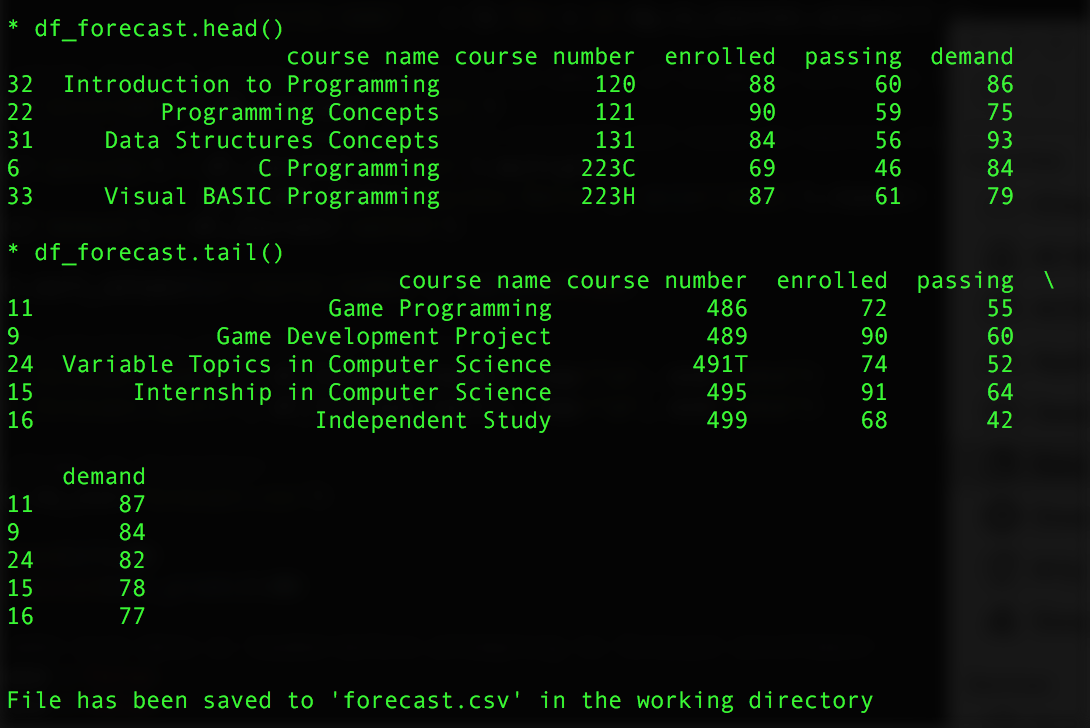
\includegraphics[scale=0.50]{result}
    \caption{Full Run}
    \label{fig:fig2}
\end{figure}


%==================== Discussion ====================

\section*{Discussion}
The course enrollment forecasting topic affects most departments in higher education. Certainly the larger ones. 
When researching this topic, little research related to individual department course forecasting was found. This 
is surprising since the forecasting topic is researched at an institution level to compute the enrollment of the incoming
class. The department offers a handbook which contains suggestions on which courses to take and at what time
to be done in a timely fashion. However, many students follow their own path which is what makes enrollment 
forecasting for a department difficult. 

There were two difficult parts when approaching this enrollment forecasting problem. First, the lack of research in 
this subject made it difficult to find an approach to improve on. Instead, it seems that to address this problem one 
will have to have an original approach which is only limited by the second difficulty, the data. As this study deals with 
student data there must be institutional review board (IRB) approval to access and use these records. For this study,
sudo records were generated however this becomes a problem when approaching the testing phase of the model.
Data is key when implementing any type of machine learning algorithm and the quality and quantity of data often
dictates the model.

Though department intuition may play a role in the final decision of how many sections and which courses should be
offered, there needs to be computational aid through some data analysis be it regression or a more advanced and 
adaptive model such as a artificial neural network.

\begin{figure}[h]
    \centering
    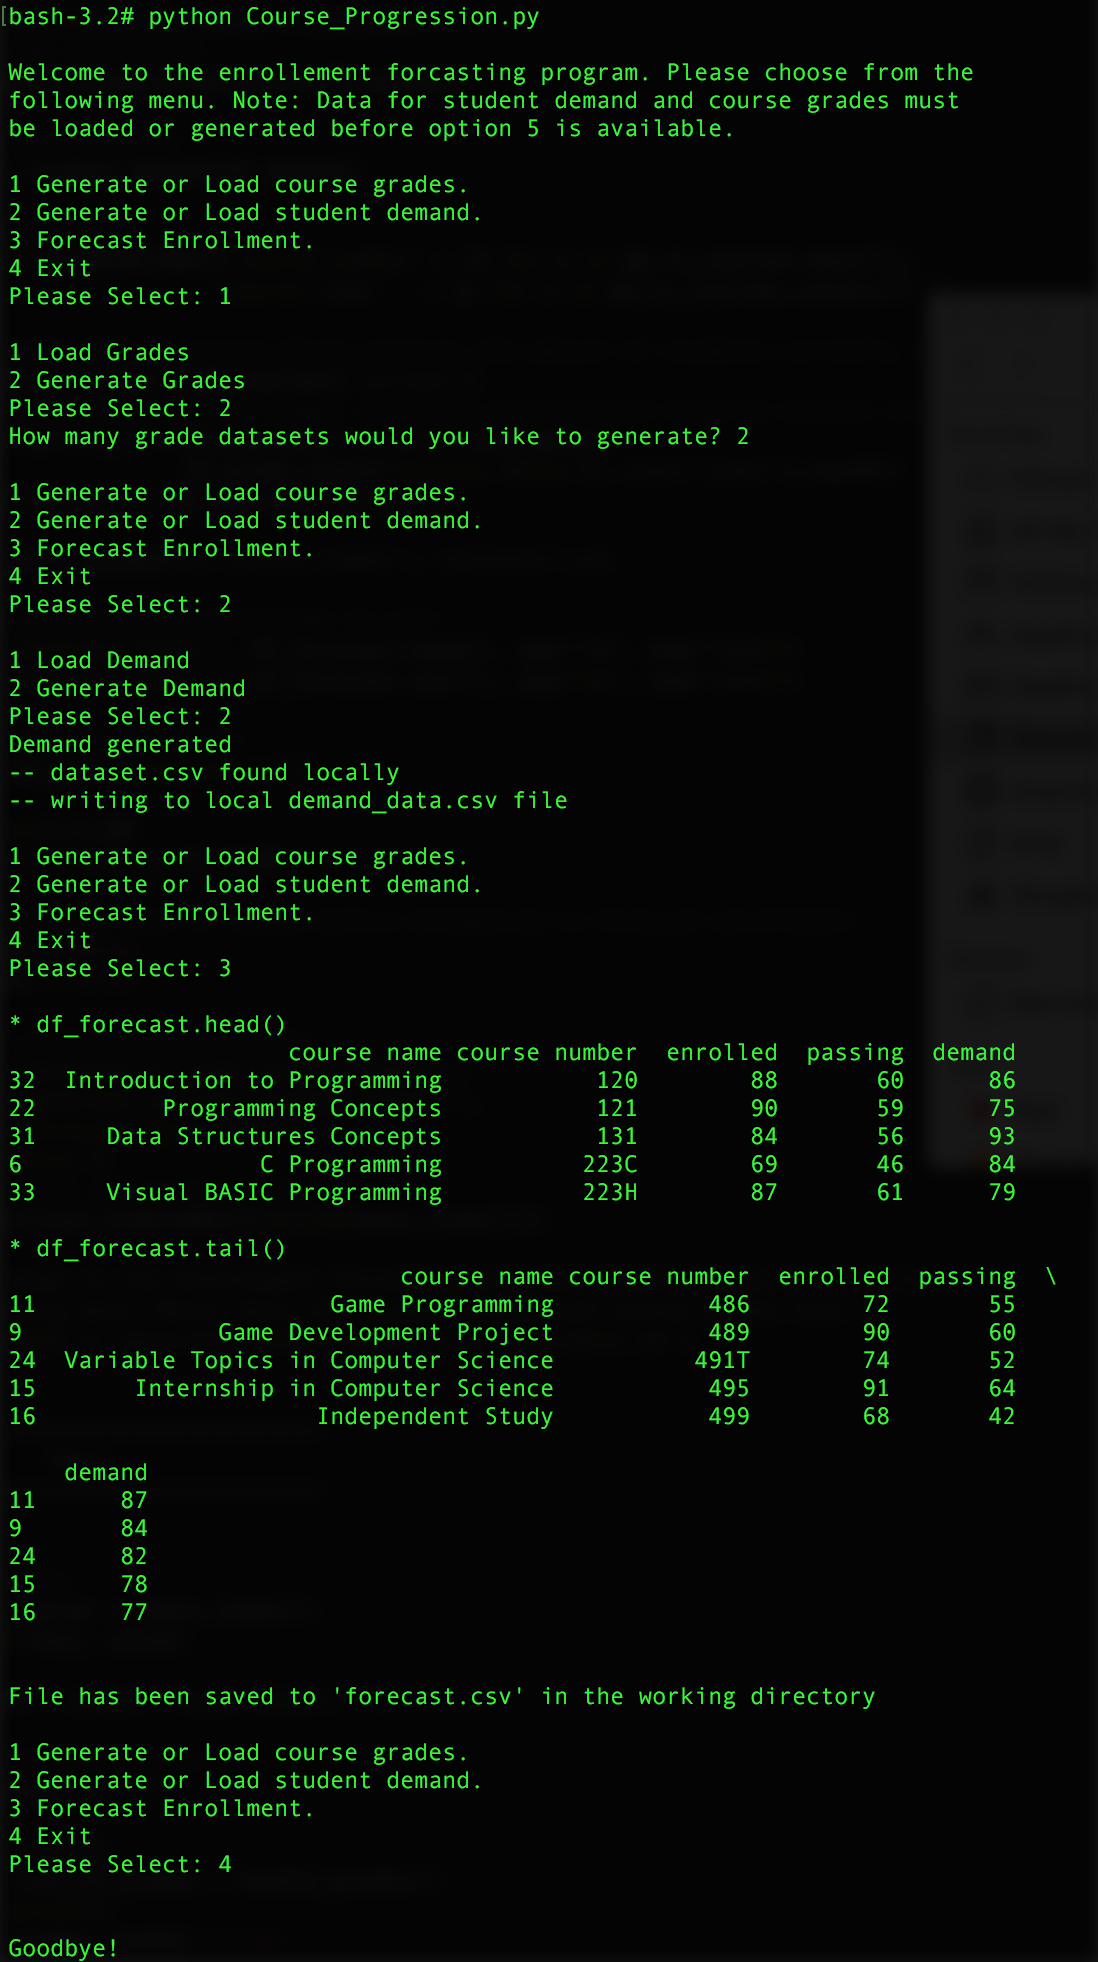
\includegraphics[scale=0.60]{fullrun}
    \caption{Full Run}
    \label{fig:fig3}
\end{figure}

\bibliography{references}

\end{document}
